\documentclass[11pt,letterpaper]{article}

\usepackage{graphicx}
\usepackage{mathpazo}

\usepackage{minted}
\usemintedstyle{arduino}

\usepackage{geometry}
\geometry{margin=1in}

\title{Delay Plot GNUPlot Output and Code}
\author{Alex Striff}
\date{August 26, 2018}

\begin{document}
\maketitle

\begin{figure}[H]
  \centering
  \colorbox{white}{%
    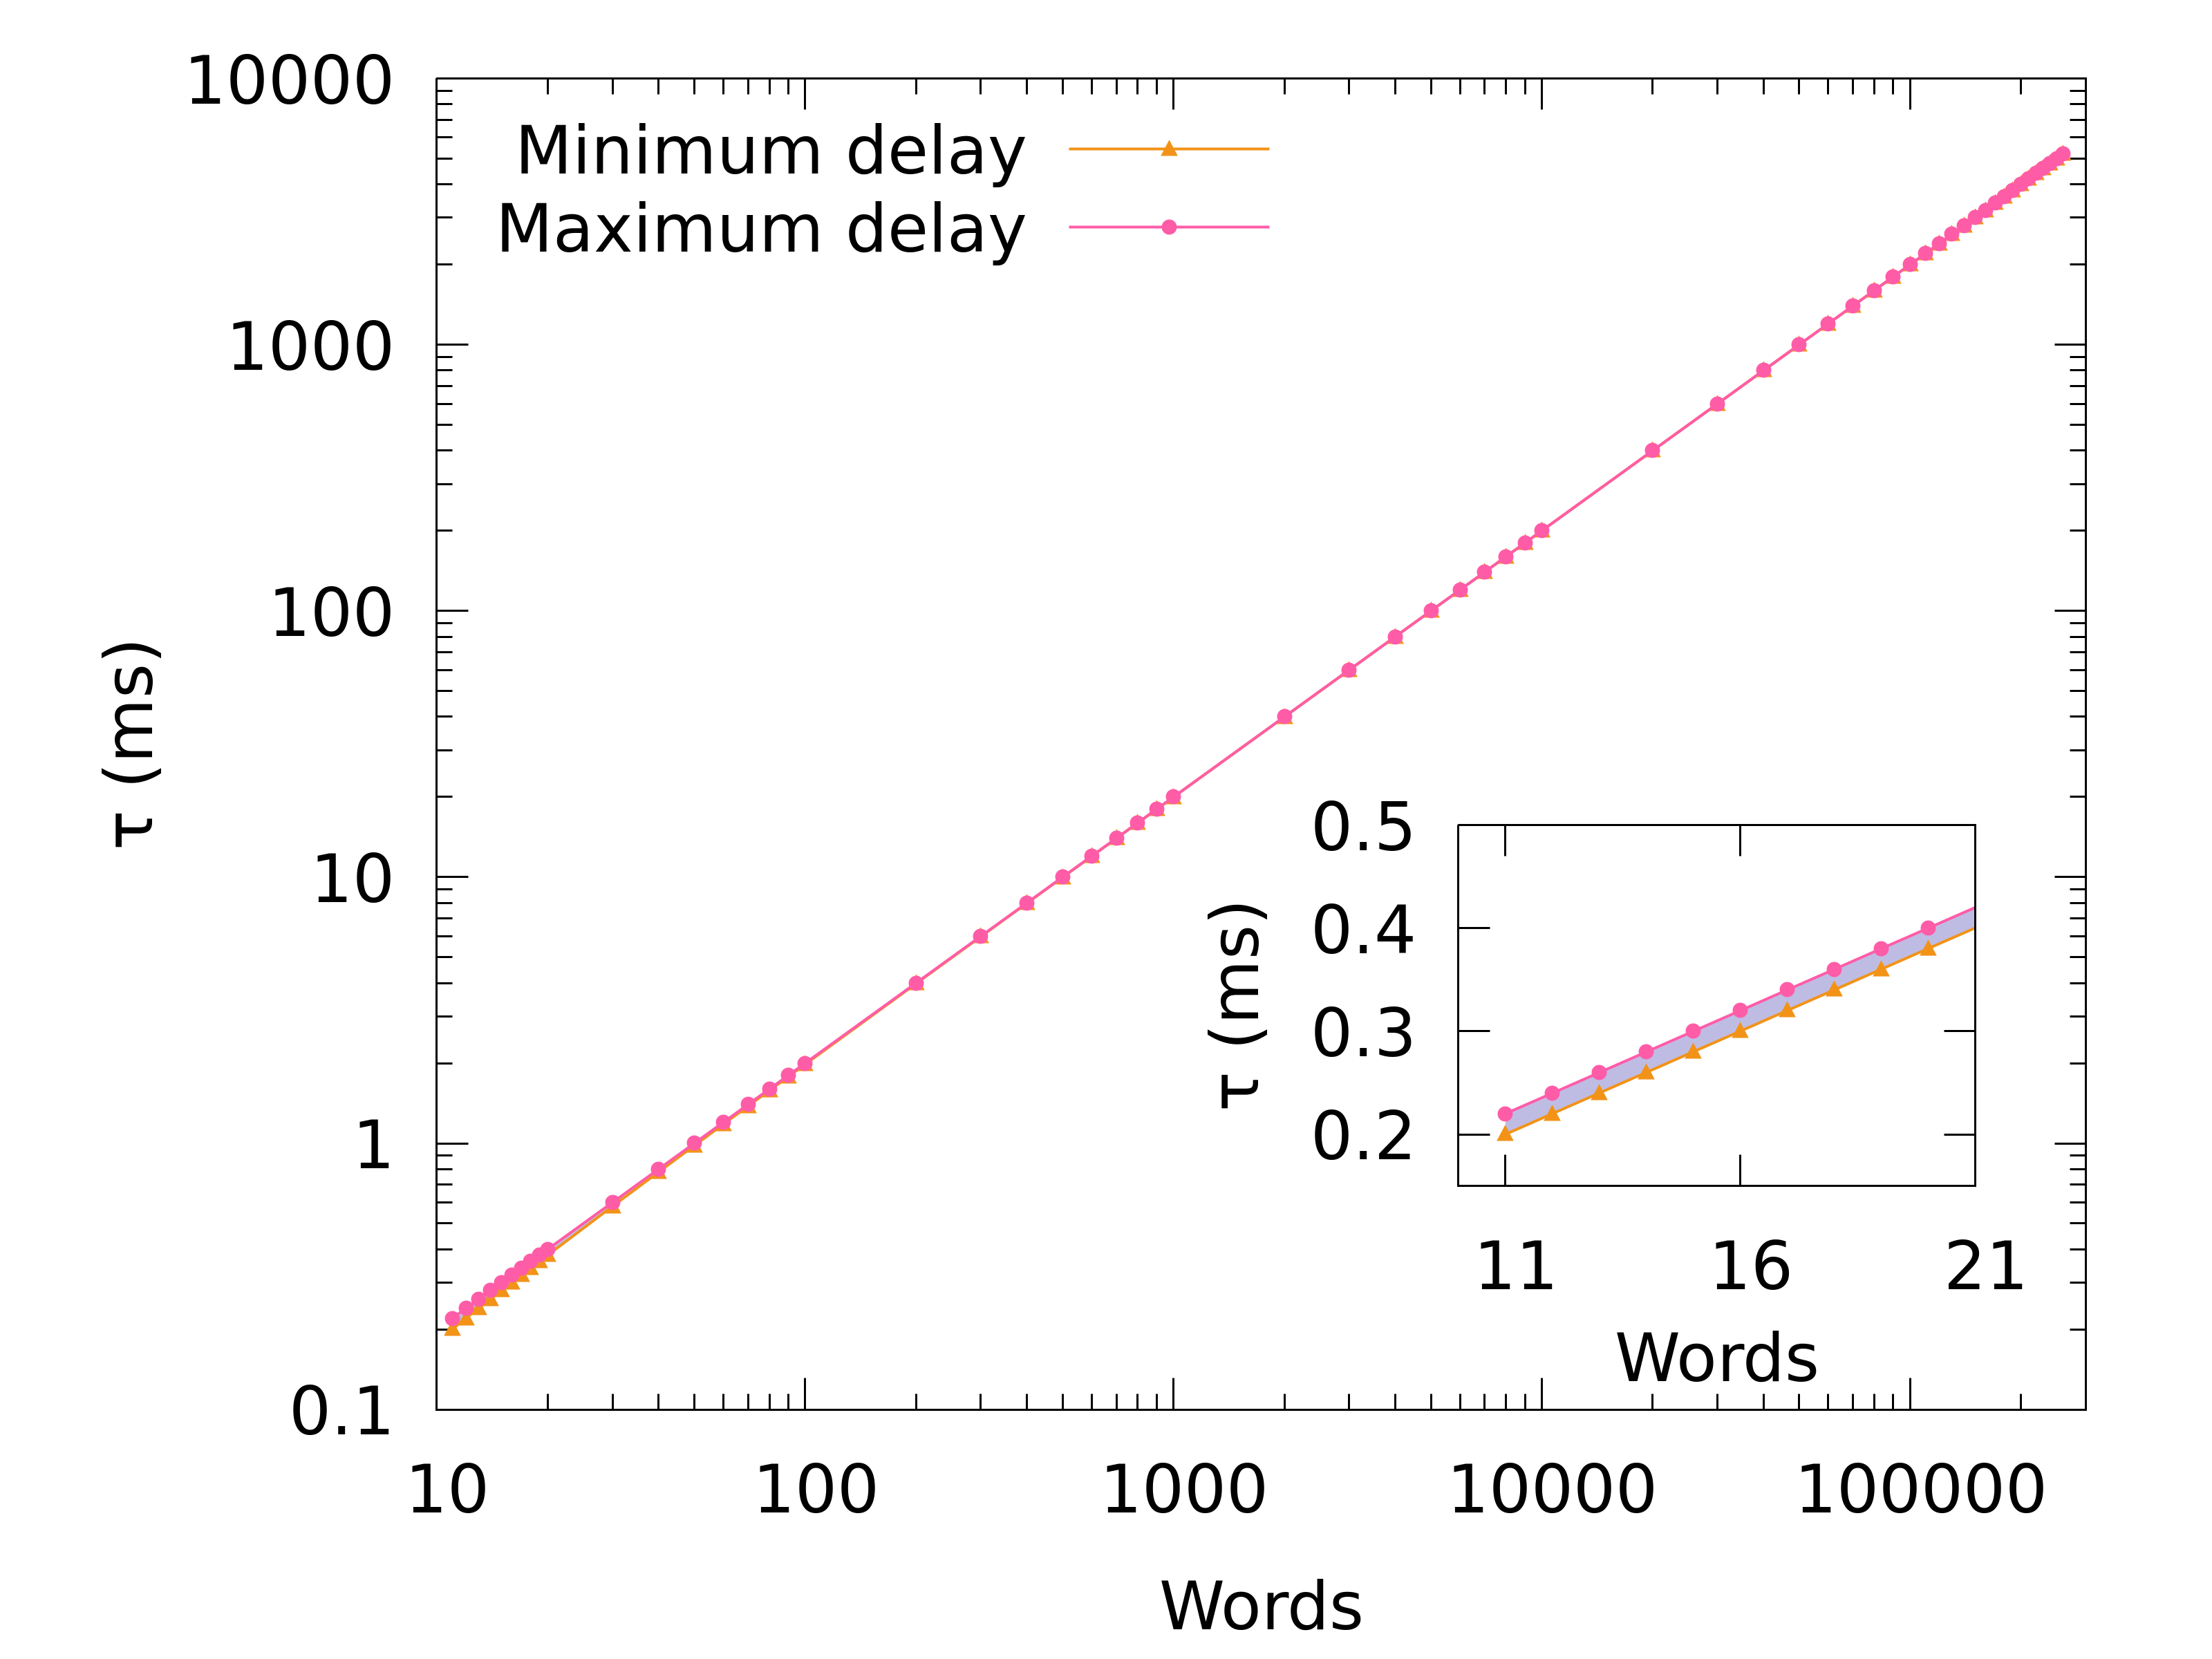
\includegraphics[width=\linewidth]{../delayplot-pc.png}
  }
  \caption{Paper, color version.}
\end{figure}
\begin{figure}[H]
  \centering
  \colorbox{white}{%
    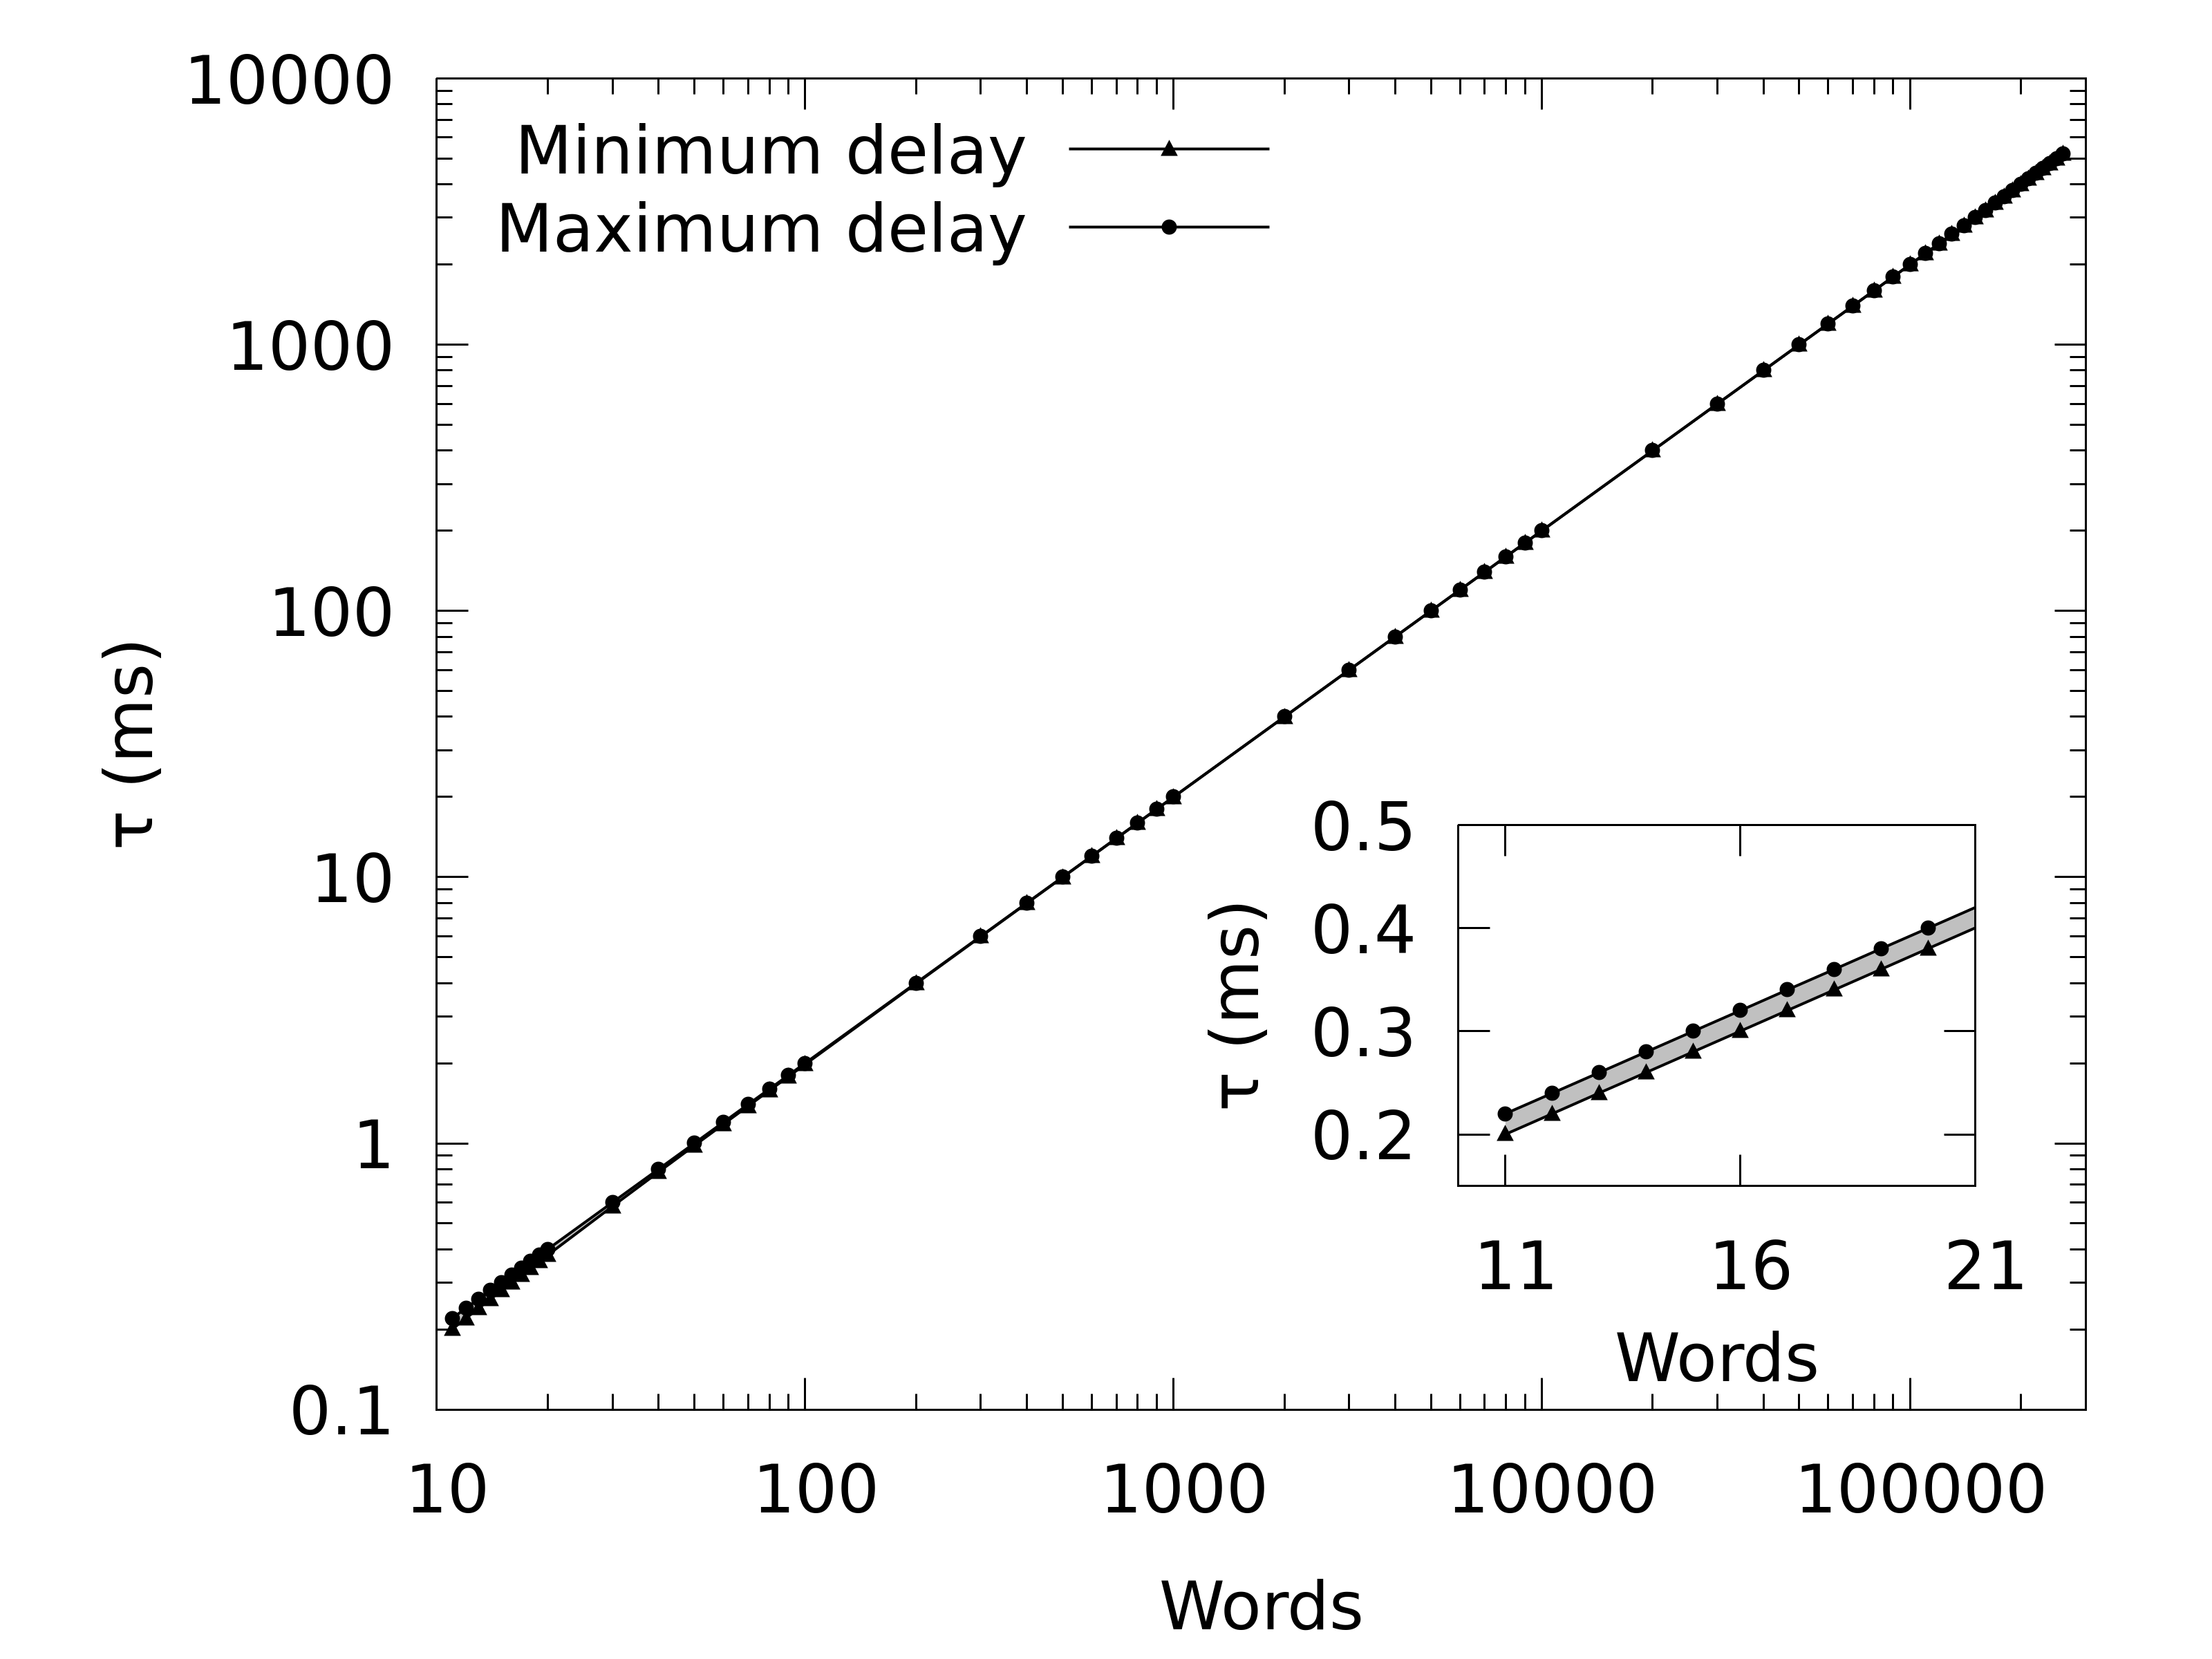
\includegraphics[width=\linewidth]{../delayplot-pg.png}
  }
  \caption{Paper, grayscale version.}
\end{figure}
\begin{figure}[H]
  \centering
  \colorbox{black}{%
    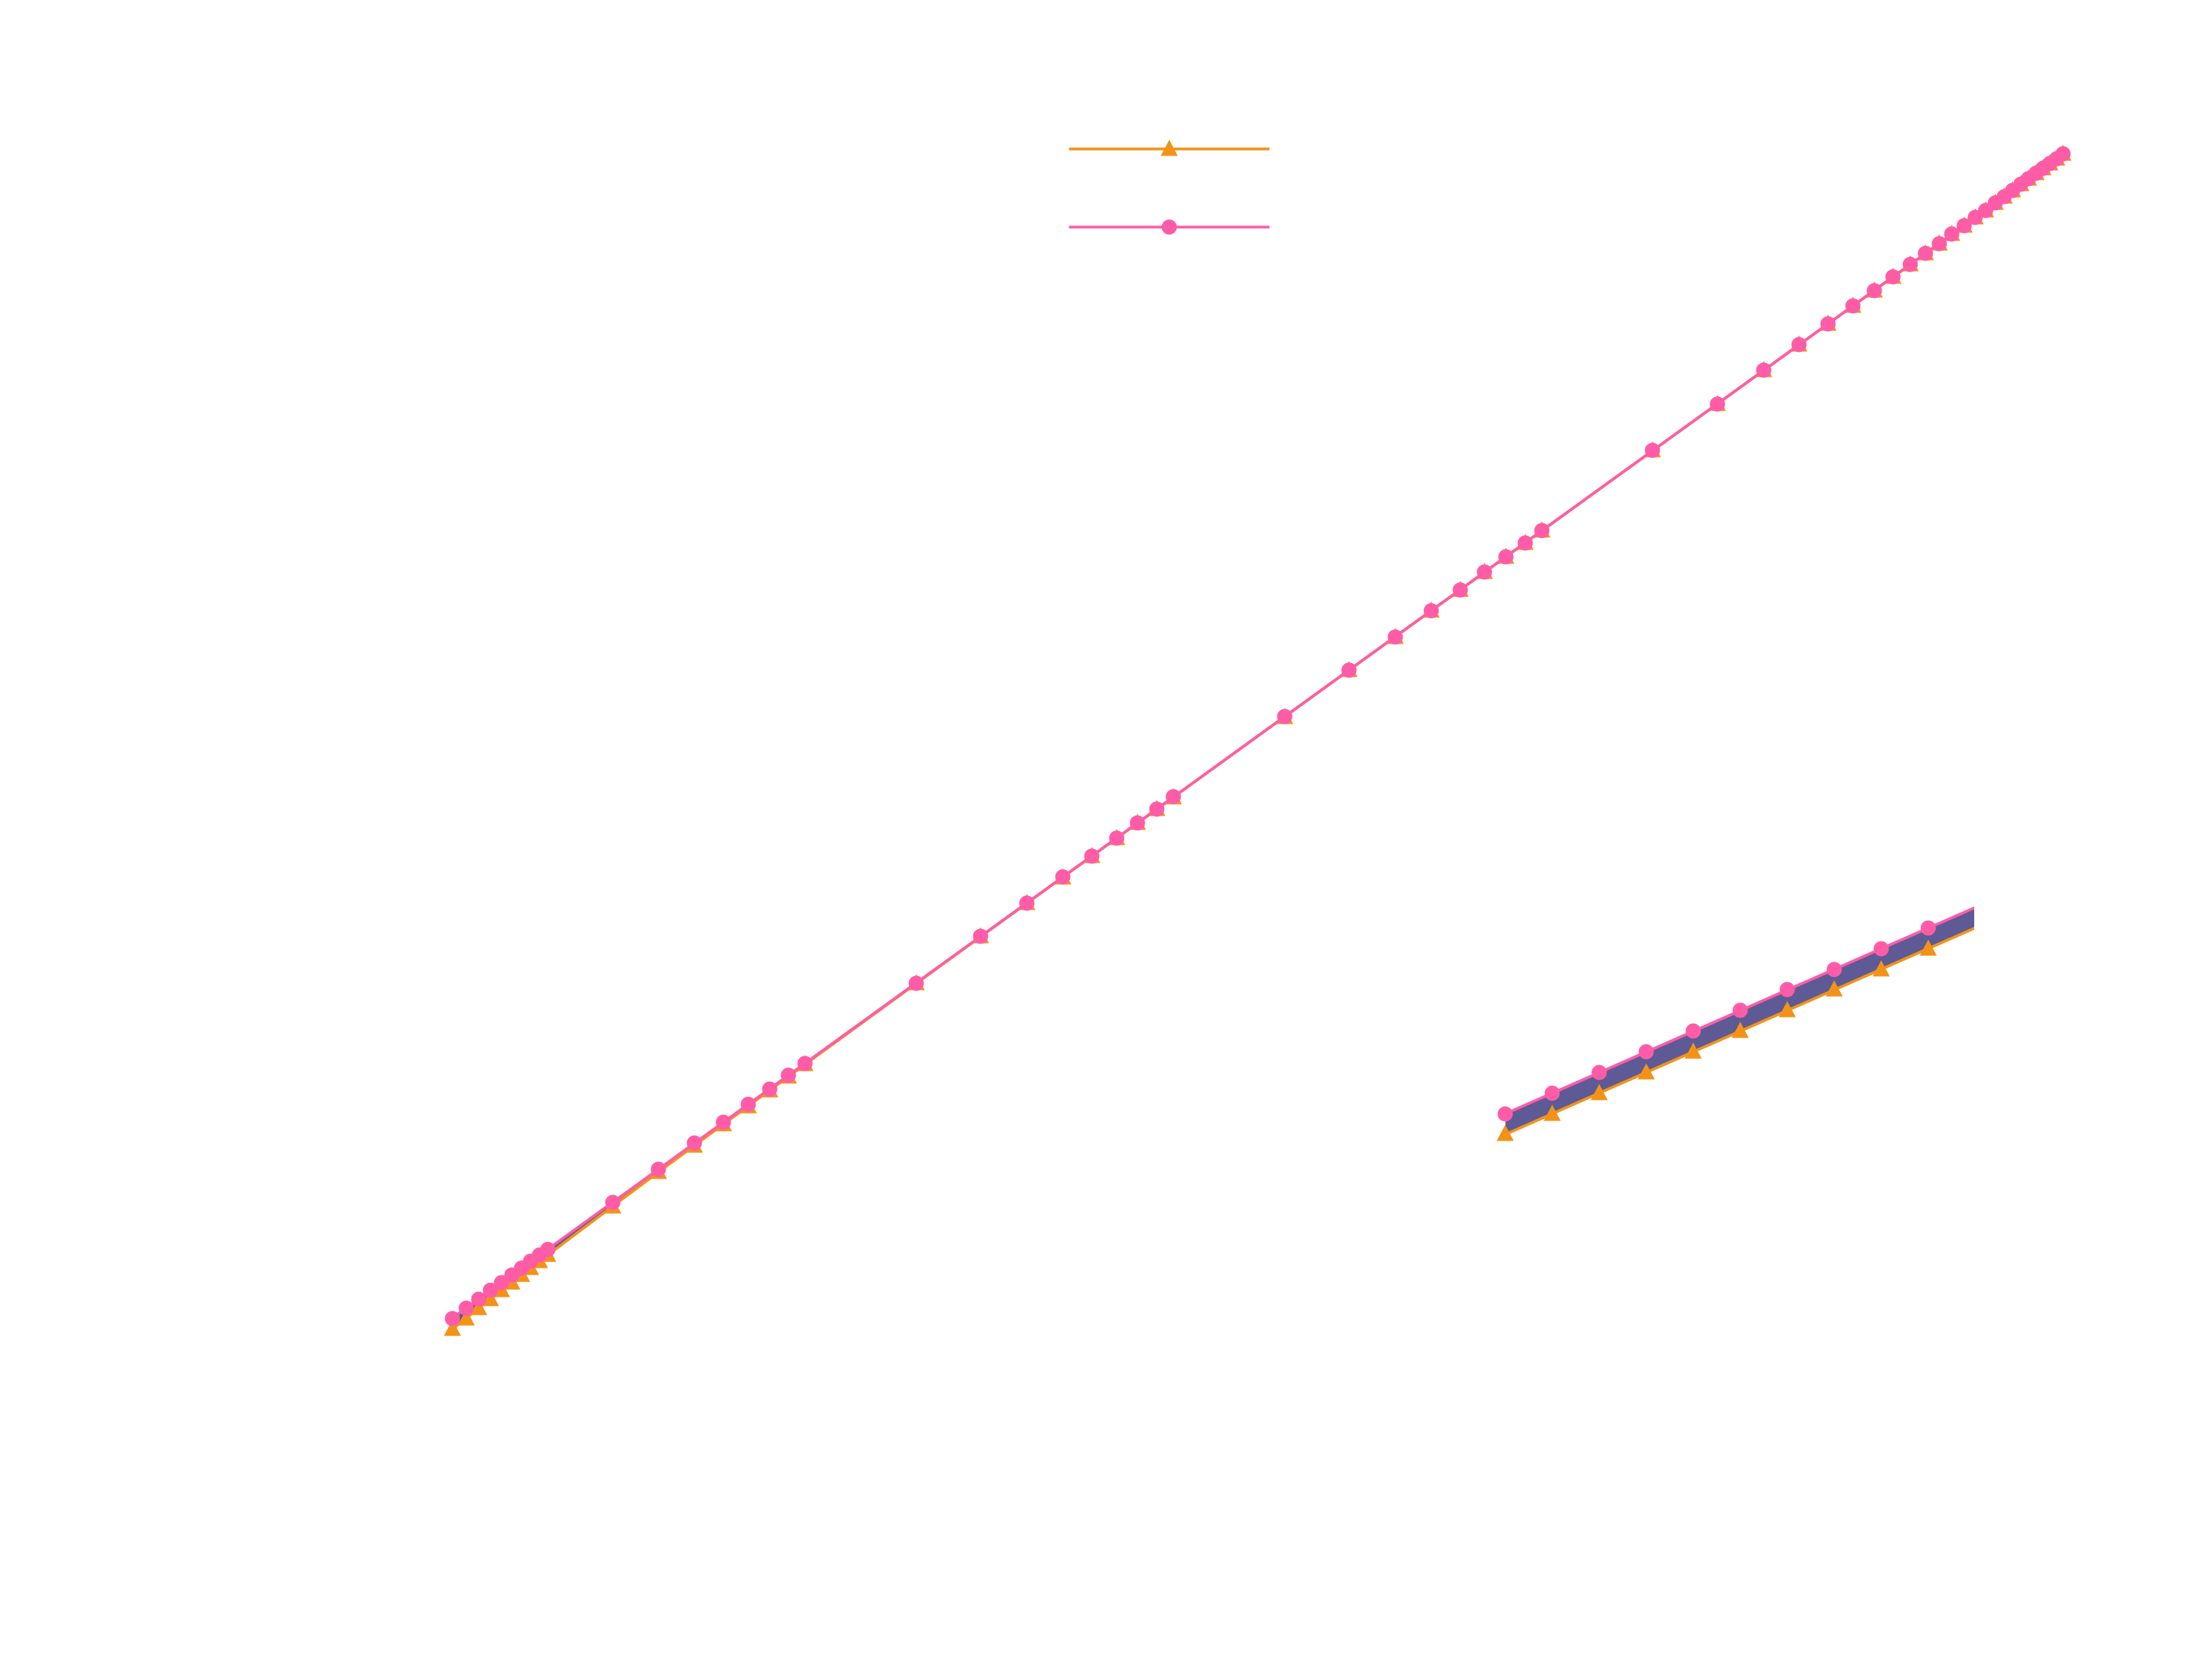
\includegraphics[width=\linewidth]{../delayplot-do.png}
  }
  \caption{Dark Owl version (beamer slides).}
\end{figure}

\begin{minted}{gnuplot}
set terminal pngcairo transparent enhanced font "Droid Sans,72" \
      fontscale 1.0 size 3200, 2400

# Dark Owl
text = '#ffffff'
shade = '#5d5a96' # (rgb(OwlRed) .+ rgb(OwlBlue)) .* 3/8
mindelay = '#f29318' # OwlYellow
maxdelay = '#ff5ca8' # OwlRed
set output 'delayplot-do.png'

# Paper Color
# text = '#000000'
# shade = '#bfbce4' # 0.25*OwlRed + 0.25*OwlBlue + 0.5*white
# mindelay = '#f29318' # OwlYellow
# maxdelay = '#ff5ca8' # OwlRed
# set output 'delayplot-pc.png'

# Paper Grayscale
# text = '#000000'
# shade = '#c0c0c0'
# mindelay = '#000000'
# maxdelay = '#000000'
# set output 'delayplot-pg.png'

set multiplot
set style increment default

set border lw 3 lc rgb text
set key tc rgb text
set xlabel tc rgb text
set ylabel tc rgb text

set datafile separator ','
dlin = 'delayplot.csv'

set origin 0,0
set size  1,1
set xtics auto
set key left top autotitle columnhead
set xlabel 'Words'
set ylabel 'τ (ms)' offset 1.5,0
set logscale xy

plot [10:3e5][] \
       dlin u 3:2:1 w filledcurves lt rgb shade t '', \
       dlin u 3:1 w linespoints pt 9 ps 3 lw 4 lc rgb mindelay t '', \
       dlin u 3:2 w linespoints pt 7 ps 3 lw 4 lc rgb maxdelay t '', \
       NaN w linespoints pt 9 ps 3 lw 4 lc rgb mindelay t 'Minimum delay', \
       NaN w linespoints pt 7 ps 3 lw 4 lc rgb maxdelay t 'Maximum delay'

set origin 0.5,0.15
set size  0.45,0.4
set xtics 11, 5
set ytics 0.1
unset key
set xlabel 'Words' offset 0,0.325
set ylabel 'τ (ms)' offset 1.5,0
unset logscale

plot [10:21][0.15:0.5] \
       dlin u 3:2:1 w filledcurves lc rgb shade, \
       dlin u 3:1 w linespoints pt 9 ps 3 lw 4 lc rgb mindelay, \
       dlin u 3:2 w linespoints pt 7 ps 3 lw 4 lc rgb maxdelay

unset multiplot

\end{minted}

\end{document}


